\documentclass{article}
\usepackage[utf8]{inputenc}

\title{CS 376 Hybrid Systems}
\author{Fred Eisele}
\date{November 2014}

\usepackage{graphicx}
\usepackage{tikz}
\usetikzlibrary{shapes,arrows}
\usepackage{amsmath}
\usepackage{amsfonts}
\usepackage{xfrac}

\begin{document}

\maketitle

\tikzstyle{block} = [draw, fill=blue!20, rectangle,
    minimum height=3em, minimum width=6em]


\section{Hybrid Timed Automaton}
Construct a timed automaton that produces $tick$
events in a periodic pattern.

\begin{equation}
1, 2, 3, 5, 6, 7 ,8, 10, 11, \ldots
\end{equation}

\ldots or the times between events \ldots

\begin{equation}
1, 1, 1, 2, 1, 1, 1, 2, 1, 1, \ldots
\end{equation}

That is three $tick$ events one second apart
and one $tick$ event two seconds later repeated.

\begin{figure}[h!]
\centering
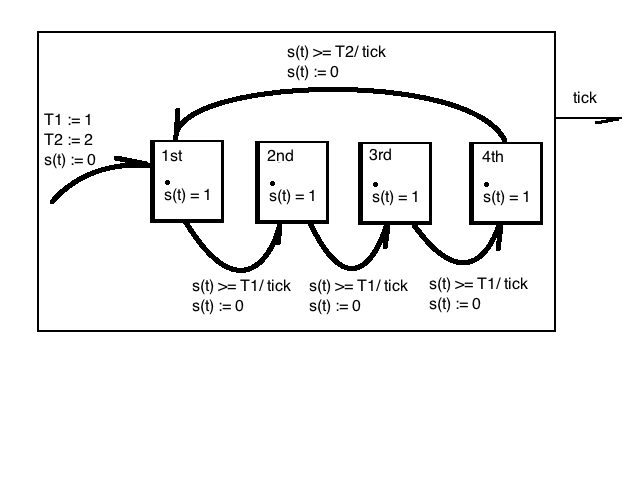
\includegraphics[scale=0.7]{hw7_1_actor_detail.png}
%% http://cremeronline.com/LaTeX/minimaltikz.pdf
\caption{Hybrid timed automata}
\label{fig:time_automata}
\end{figure}

The formal model is that of a hybrid automaton.
The formal model for the hybred atutomaton presented in
class differs slightly from the one implicit in the textbook.
The textbook allows for signals on the guard and constants.
There are also two constants $T_1 = 1$ and $T_2 = 2$.

\begin{equation}
H = (Q, X, O, Init, f, Inv, E, G, R)
\end{equation}

The set of discrete variables.
\begin{equation}
Q & = \{1st, 2nd, 3rd, 4th\}
\end{equation}

The set of continuous variables.
$X = \mathbb{R}$
\begin{equation}
X = \{s(t)\}
\end{equation}

The set of output signals.
\begin{equation}
O = \{ tick \} : \text{pure}
\end{equation}

The set of initial conditions.
$Init \subseteq Q \times X$
\begin{equation}
Init = \{ ( 1st, s(t)} := 0 ) \}
\end{equation}

The vector field.
$f: Q \times X$
\begin{align}
f = \{ & ( 1st, \dot{s(t)} = 1 ) \\
    & ( 2nd, \dot{s(t)} = 1 ) \\
    & ( 3rd, \dot{s(t)} = 1 ) \\
    & ( 4th, \dot{s(t)} = 1 ) \}
\end{align}

The invariant set. (all empty)
$Q \mapsto 2^X$
\begin{align}
Inv = \{ & ( 1st, \emptyset ) \\
    & ( 2nd, \emptyset ) \\
    & ( 3rd, \emptyset ) \\
    & ( 4th, \emptyset ) \}
\end{align}

The collection of discrete transitions.
$E \subset Q \times Q$
\begin{align}
E = \{ & ( 1st, 2nd ) \\
    & ( 2nd, 3rd ) \\
    & ( 3rd, 4th ) \\
    & ( 4th, 1st ) \}
\end{align}

The guards on the transitions.
This makes an accomdation for signals,
this could be emulated with a continuous variable
but the problem specification calls for a signal.
$G: E \mapsto (2^X / O)$
\begin{align}
G = \{ & (( 1st, 2nd ), (s(t) >= T_1 / tick ) \\
    & (( 2nd, 3rd ), (s(t) >= T_1 / tick ) \\
    & (( 3rd, 4th ), (s(t) >= T_1 / tick ) \\
    & (( 4th, 1st ), (s(t) >= T_2 / tick ) \}
\end{align}

The reset relation on the transitions.
$R: E \times X \mapsto 2^X$
\begin{align}
R = \{ & (( 1st, 2nd , s(t)),  0 ) \\
    & (( 2nd, 3rd , s(t)), 0 \\
    & (( 3rd, 4th , s(t)), 0  \\
    & (( 4th, 1st , s(t)), 0  \}
\end{align}

\section{Automobile Features}

\subsection{Dome Light}
The dome light is turned on as soon as any door
is opened.
It stays on for 30 seconds after all doors are shut.
A sensor which can detect when a door's position,
$\{opened, closed\}$ is needed for each door.
I have modeled this automaton with sensors that
produce signals.
I could have used a separate continuous variable
for each door sensor, which would have resulted
in a different model.
The light invariant is not strictly necessary but
it emphasizes the fact that the light should be on
when any of the doors are open.

\begin{figure}[h!]
\centering
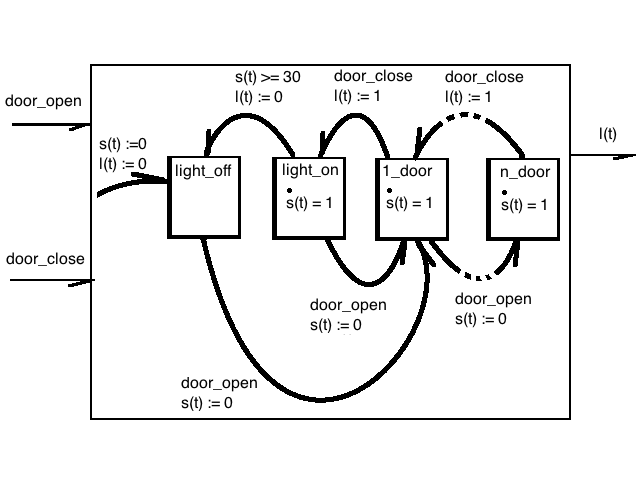
\includegraphics[scale=0.7]{hw7_4a_actor_dome.png}
\caption{A dome light}
\label{fig:dome_light}
\end{figure}


The formal model is that of a hybrid automaton
augmented with signals.
\begin{equation}
H = (Q, X, O, Init, f, Inv, E, G, R)
\end{equation}

The set of discrete variables.
\begin{equation}
Q & = \{light_{off}, light_{on}, door_1, door_2, \ldots, door_n \}
\end{equation}
The light is off and all the doors are closed.

The set of continuous variables.
$X = \mathbb{R}$
\begin{equation}
X = \{ s(t), l(t) \}
\end{equation}

The set of signals.
\begin{equation}
O = \{ door_{open}, door_{close} \}
\end{equation}

The set of initial conditions.
$Init \subseteq Q \times X$
\begin{equation}
Init = \{ ( light_{off}, l(t) := 0 , s(t) := 0) \}
\end{equation}

The vector field.
$f: Q \times X$
\begin{align}
f = \{ & ( light_{on}, { \dot{s(t)} = 1 } )  \}
\end{align}

The invariant set.
$Q \mapsto 2^X$
\begin{align}
Inv = \{
    & ( light_{on}, { l(t) = 1 } ) \\
    & \ldots \\
    & ( door_n, { l(t)} = 1}) \}
\end{align}

The collection of discrete transitions.
$E \subset Q \times Q$
\begin{align}
E = \{
    & ( light_{off}, door_1 ) \\
    & ( light_{on}, door_1 ) \\
    & ( door_1, door_2 ) \\
    & \ldots \\
    & ( door_{n-1}, door_n ) \\
    & ( door_n, door_{n-1} ) \\
    & \ldots \\
    & ( door_2, door_1 ) \\
    & ( door_1, light_{on} ) \\
    & ( light_{on}, light_{off} ) \}
\end{align}

The guards on the transitions.
These guards also take signals in addition to
predicates over the continuous variables.
$G: E \mapsto 2^X$
\begin{align}
G = \{ & ( light_{off}, door_1 ) \mapsto door_{open} \\
    & ( light_{on}, door_1 ) \mapsto door_{open} \\
    & ( door_1, door_2 ) \mapsto door_{open} \\
    & \ldots \\
    & ( door_{n-1}, door_n ) \mapsto door_{open} \\
    & ( door_n, door_{n-1} ) \mapsto door_{close} \\
    & \ldots \\
    & ( door_2, door_1 ) \mapsto door_{close} \\
    & ( door_1, light_{on} ) \mapsto door_{close} \\
    & ( light_{on}, light_{off} \mapsto s(t) \geq 30 ) \}
\end{align}

The reset relation on the transitions.
$R: E \times X \mapsto 2^X$
\begin{align}
R = \{ & ( light_{off}, door_1 ) \mapsto l(t) := 1 \\
    & ( light_{on}, door_1 ) \mapsto  l(t) := 1 \\
    & ( door_1, light_{on} ) \mapsto s(t) := 0 \\
    & ( light_{on}, light_{off} \mapsto l(t) := 0 ) \}
\end{align}

\subsection{Safety Belt Alarm}
Once the engine is runing,
a beeper is sounded and
a red light warning is indicated if thre are
passengers that have not buckled their seat belt.
The beeper stops sounding after 30 seconds, or
as soon as the seat belts are buckled,
whichever is sooner.
The warning light remains on so long as the
seatbelt on an occupied seat is not buckled.

The problem is made more tractable by
replacing the engine running condition with
the ignition on condition (for gasoline engines
this is a reasonable assumption).

Each seat has two sensors, one indicating that
the $seat \in \{occupied_i ,empty_i\}$
and one indicating that the
$seatbelt \in \{buckled_i, unbuckled_i\}$.
Another sensor indicates
$ignition \in \{on, off\}$

The actuators are controlled by continuous variables,
$light_{warning}$ as $l(t)$ and
$beeper_{warning}$ as $b(t)$.

There are some assumptions in play.
$warn$ \is an event generated when the $ignition$ is
turned $on$ and any $seat$ is $occupied$ or when
the $ignition$ is already $on$ and a $seat$ becomes
occupied.

The formal model is that of a multi-agent hybrid automaton.
The formal model is not required for the assignment
and sections will be omitted.
Some sections will be included sufficient to define terms.

\begin{equation}
H = (Q, X, O, Init, f, Inv, E, G, R)
\end{equation}

The set of discrete variables.
\begin{align}
Q_{total} & = \{clear, beep, light \} \\
Q_{seat} & = \text{the states that a seat can take} \\
Q_{aggregate} & = \text{the aggregate seat states} \\
Q & = Q_{total} \cup Q_{seat}^n \cup Q_{aggregate}
\end{align}
Here the $n$ seats are indexed by $i$.

First the output variables to the actuators.
\begin{align}
light_{warn} : l(t) & =
   \begin{cases}
      0, & \text{warning light off} \\
      1, & \text{warning light on}
    \end{cases} \\
 beep_{warn} : b(t) & =
   \begin{cases}
      0, & \text{warning beeper off} \\
      1, & \text{warning beeper on}
    \end{cases}
\end{align}

And, the continuous variables from input sensors.
\begin{align}
 ignition : e(t) & =
   \begin{cases}
      0, & \text{ignition off} \\
      1, & \text{ignition on}
    \end{cases} \\
  belt : f(t,i) & =
   \begin{cases}
      0, & \text{unbuckled} \\
      1, & \text{buckled}
    \end{cases} \\
  seat : s(t,i) & =
   \begin{cases}
      0, & \text{empty} \\
      1, & \text{occupied}
    \end{cases}
\end{align}

Giving us the set of continuous variables.

The set of continuous variables.
$X = \mathbb{R}$
Notice that $n$ seats/seatbelts are accomdated and indexed by $i$.
The system state comprises the following elements.
\begin{equation}
 X = (e(t), r(t), (f(t,i), s(t,i))^n)
\end{equation}


The model consists of three types of connected agent models.

$noWarn$ is an event generated when a $seatbelt$ is $buckled$
a $seat$ becomes $empty$ or the $ignition$ is turned $off$.

\begin{figure}[h!]
\centering
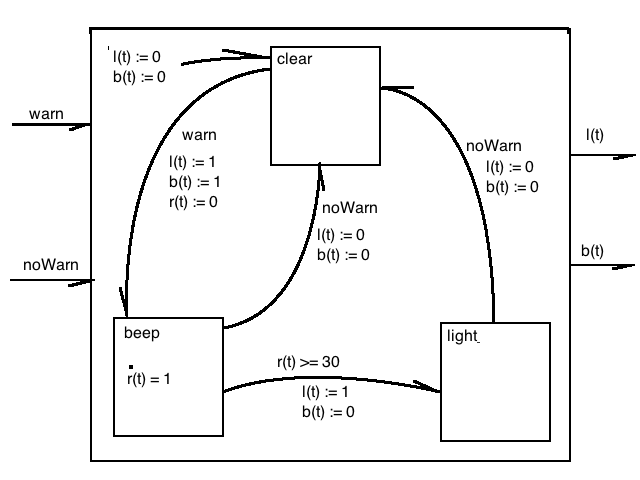
\includegraphics[scale=0.7]{hw7_4b_actor_total.png}
\caption{The final actor}
\label{fig:4b_actor_total}
\end{figure}

I have not place any invariants in this model.
They could be added to the $beep$ mode to indicate
that the light is $on$ ($l(t) = 1$) and to the $light$ mode to
indicate that the $beeper$ is $off$ ($b(t) = 0$).
Similarly, in the $clear$ mode they are both $off$.
However, this is redundant information so I left
them off the diagram.


The $warn$ and $noWarn$ inputs to the total model are
produced by an aggregation agent with combines the
events for the individual $seats_i$ which have corresponding
$warn_i$ and $noWarn_i$ variables.

If a $warn$ is received in either the $light$ or $beep$
mode there is no change in mode, according to
 the assumptions.

\begin{figure}[h!]
\centering
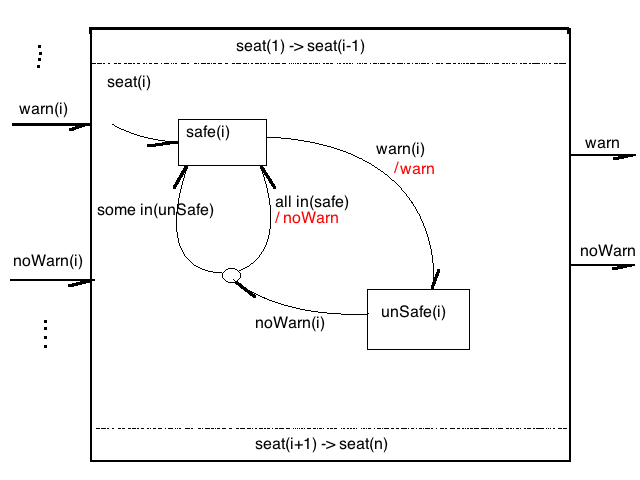
\includegraphics[scale=0.7]{hw7_4b_actor_aggr.png}
\caption{The aggregate actor}
\label{fig:4b_actor_aggr}
\end{figure}


Feeding into the aggregator agent are $n$ seats.

\begin{figure}[h!]
\centering
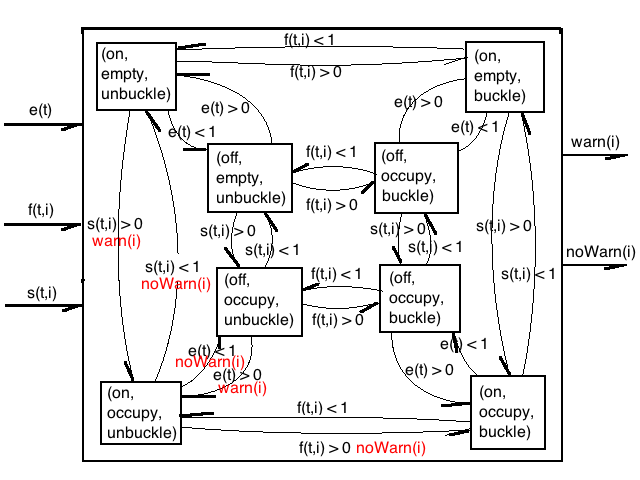
\includegraphics[scale=0.7]{hw7_4b_actor_seat.png}
\caption{A seat actor}
\label{fig:4b_actor_seat}
\end{figure}


\end{document}
